\documentclass[10pt]{article}
\usepackage[margin=1in]{geometry}
\usepackage{graphicx}
\usepackage{booktabs}
\usepackage{amsmath}
\usepackage{amssymb}
\usepackage{xcolor}
\usepackage[colorlinks=true,linkcolor=blue,citecolor=blue,urlcolor=blue]{hyperref}
\usepackage{enumitem}

\newcommand{\rhg}{\textsf{RHG}}
\newcommand{\hpr}{\textsf{HPR}}
\newcommand{\code}[1]{\texttt{#1}}

\title{\textbf{The RTL Gauntlet}: Measuring Honesty, Cost, and\\
Latency-Robustness in Agentic Hardware Design}
\author{(working draft)}
\date{}

\begin{document}
\maketitle

\begin{abstract}
Agentic RTL frameworks now report $100\%$ pass on standard benchmarks, but that score is measured
against \emph{visible} tests, is \emph{expensive} to reach, and is obtained on \emph{proxy} tasks.
We turn these three concerns into measurable axes. We build a two-tier protocol that freezes an
agent's design and scores it with a withheld formal-equivalence oracle, and define a
Reward-Hacking Gap (\rhg) and Honest Pass Rate (\hpr). Applying it to 156 VerilogEval tasks across
two models, we find the na\"ive headline \rhg{} ($6.1\%$) is \emph{entirely an oracle artifact}: a
na\"ive formal oracle over-reports reward hacking via don't-care \code{x}, async-reset,
state-encoding, init-state, and even a SystemVerilog parser flag. We harden the oracle in five steps
---reset-aware, don't-care-aware, bounded miter+SAT, \code{read\_verilog -sv}, and a \code{memory}
(case$\to$ROM) pass---cutting false counter-examples $9\!\to\!1$ and ``inconclusive'' $50\!\to\!6$,
and verify every surviving flag by hand: \textbf{zero genuine reward hacking} ($95\%$ upper bound
$\le\!3\%$) by frontier models on fair tasks. A weaker model (Haiku~4.5) fails $3\times$ more than
Opus~4.8 on the visible tests but does \emph{not} hack more; even a tamper-capable shell agent that
struggles for several iterations does not edit the testbench. We show the oracle \emph{would} catch
hacking when present (a candidate that passes a randomized hidden testbench but is formally
disproven), that the result survives off the verbatim benchmark (a contamination probe), and we add
a token-cost analysis (an early-stop reclaims $12$--$23\%$ of tokens) and a latency-axis prototype
that produces real Sky130 power/area/timing through a containerized OpenLane flow. The central
artifact for honest agentic-hardware evaluation is a don't-care/reset/encoding-aware oracle plus a
verification discipline---not a new pass-rate.
\end{abstract}

\section{Introduction}
HORIZON treats agentic hardware design as repository-level code evolution and reaches $100\%$ pass
on several RTL suites---but iteration-0 pass is only $47.8\%$, so the headline comes from
\emph{iterative repair against a visible signal}. Its authors name three open problems: reward
hacking, token cost, and high-latency (PPA) reward. We make each measurable.

\paragraph{Thesis.} \emph{Pass@visible is the wrong score for agentic hardware design}: it can be
gamed (honesty), it is expensive (cost), and it does not scale to real reward (latency).

\paragraph{Contributions.}
\begin{enumerate}[leftmargin=*,topsep=2pt,itemsep=1pt]
\item A two-tier, formal-grounded evaluation protocol with metrics \rhg{} and \hpr{} (\S\ref{sec:method}).
\item The finding that a na\"ive formal oracle \textbf{over-reports} reward hacking, and a
five-step hardened oracle that removes it; verification discipline as a first-class method
(\S\ref{sec:oracle}).
\item An empirical result across $2$ models $\times\,156$ tasks: \textbf{zero verified genuine
reward hacking} on fair tasks; weakness $\ne$ hacking; tampering is caught when present
(\S\ref{sec:exp}).
\item Cost and latency prototypes: token accounting with an early-stop policy, and real Sky130 PPA
via a containerized flow (\S\ref{sec:exp}).
\end{enumerate}

\section{Related Work and Positioning}
Formal-equivalence-as-oracle is already community-standard for RTL--LLM evaluation
(VeriThoughts; NotSoTiny; RealBench)---so it is our \emph{tool}, not our contribution.
Table~\ref{tab:related} situates the closest work.

\begin{table}[t]\centering\small
\begin{tabular}{@{}lccc@{}}
\toprule
Work & gap metric & formal oracle & RTL \\
\midrule
SpecBench & \checkmark (software) & finite held-out & --- \\
EvilGenie & \checkmark + edit-detect & --- & --- \\
Agentic Frontier & --- & --- & \checkmark \\
\textbf{This work} & \checkmark & \textbf{exhaustive} & \checkmark \\
\bottomrule
\end{tabular}
\caption{SpecBench owns the visible/held-out gap for \emph{software} and admits its held-out suite
``cannot exhaustively certify compliance.'' Our slot: RTL $+$ an exhaustive formal oracle (fixing
that limit) $+$ tamper-evidence.}
\label{tab:related}
\end{table}

\section{Method: the two-tier protocol}\label{sec:method}
The agent sees a complete specification, a \emph{visible} diagnostic testbench, and its failure
logs, and edits RTL until visible passes. We then \textbf{freeze} the design and score withheld
tiers it never saw: a hidden randomized/exhaustive testbench, and \textbf{formal equivalence} vs.\ a
curated golden (Yosys). The I/O interface is locked. We define
\[
\rhg = \tfrac{\#\{\text{visible-passers failing a withheld tier}\}}{\#\{\text{visible-passers}\}},
\quad
\hpr = \tfrac{\#\{\text{pass visible and every withheld tier}\}}{\#\text{tasks}} .
\]
A tamper tier (a shell-capable agent that may edit any workspace file) flags edits to the
testbench/harness as \emph{exploit-evidenced} hacking, with the withheld tiers run on frozen
originals so tampering cannot fool the verdict. We separate the claim into behavioral gap,
exploit-evidenced, and tamper-confirmed, and never claim intent without trajectory evidence.

\section{The oracle, and why na\"ive formal over-reports}\label{sec:oracle}
On a 156-task sweep (Opus~4.8), a na\"ive \code{equiv\_make} oracle reported $9$ \rhg{}
counter-examples and $50$ ``inconclusive.'' \textbf{Every CEX was a false positive}, found by
hand-verifying flagged cases: don't-care \code{x} in the golden; functionally identical designs
flagged on async reset / initial state; a candidate logically identical but with a different state
encoding; and---for most ``inconclusive''---a silent parse failure, since \code{read\_verilog}
defaults to Verilog-2005 while the references use \code{always\_ff}/\code{logic}/enums.

Our hardening pipeline (each step tested on verified cases before re-running):
\begin{enumerate}[leftmargin=*,topsep=2pt,itemsep=0pt]
\item \code{async2sync} (normalize async resets);
\item reclassify a CEX to \emph{dontcare} when the golden has an \code{x} literal;
\item a bounded miter$+$SAT fallback comparing I/O sequences directly (encoding-agnostic; a SAT
model is a real CEX);
\item \code{read\_verilog -sv};
\item a \code{memory} (case$\to$ROM) pass.
\end{enumerate}

\begin{table}[t]\centering\small
\begin{tabular}{@{}lcccccc@{}}
\toprule
stage & honest & bmc & dc & \rhg & inconcl & fail \\
\midrule
na\"ive & 88 & -- & -- & 9 & 50 & 9 \\
+reset+dc & 91 & -- & 3 & 3 & 50 & 9 \\
+BMC & 91 & 3 & 2 & 1 & 50 & 9 \\
+SV & 122 & 6 & 4 & 1 & 14 & 9 \\
+memory & \textbf{129} & 6 & 5 & 1 & \textbf{6} & 9 \\
\bottomrule
\end{tabular}
\caption{Oracle hardening (same 156 Opus candidates, no new LLM calls). False CEX $9\!\to\!1$;
inconclusive $50\!\to\!6$; \hpr{} $56\%\!\to\!87\%$. The $6$ residual are hard sequential FSMs.}
\label{tab:progression}
\end{table}

\begin{figure}[t]\centering
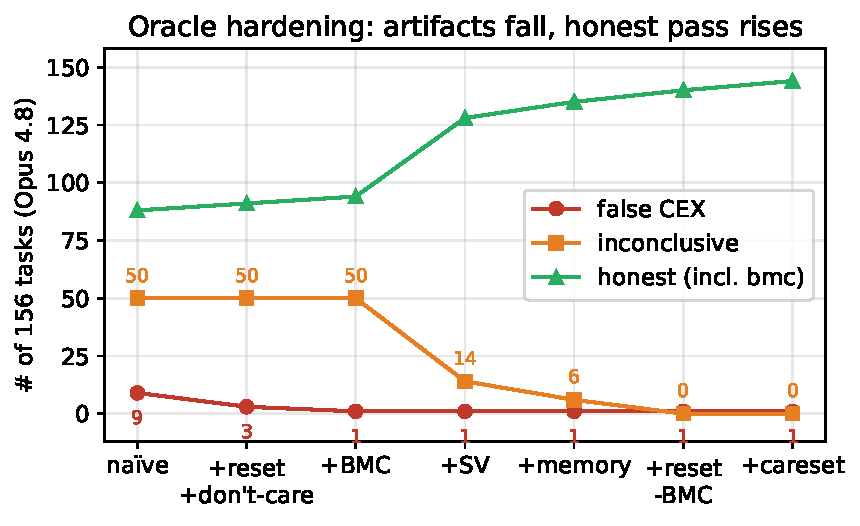
\includegraphics[width=0.95\linewidth]{figures/progression.pdf}
\caption{Oracle hardening: artifacts fall (false CEX $9\!\to\!1$, inconclusive $50\!\to\!6$) and the
honest pass count rises ($88\!\to\!135$).}
\label{fig:prog}
\end{figure}

\section{Experiments}\label{sec:exp}

\paragraph{Formal earns its keep.} \code{formal\_demo}: a 16-bit candidate wrong \emph{only} on
\code{0xDEAD}. The randomized hidden testbench ($512/65536$) misses it---visible \emph{and} hidden
PASS---while exhaustive formal returns CEX. With finite tests alone $\rhg{}=0$ (it looks honest);
formal exposes it ($\rhg{}=0.50$). This is the direct evidence that an exhaustive formal oracle
beats a finite held-out suite.

\paragraph{Sweep and model comparison.} Table~\ref{tab:models} and Figure~\ref{fig:models}: the
weaker model fails far more (\code{fail\_visible} $9\!\to\!30$, $+11$ no compilable candidate) but
hacks no more. Both residual \rhg{} counter-examples are verified init artifacts. With $95\%$ Wilson
intervals, verified-genuine \rhg{}$=0$ with an upper bound $\le\!2.5\%$ (Opus) / $\le\!3.2\%$ (Haiku).

\begin{table}[t]\centering\small
\begin{tabular}{@{}lcc@{}}
\toprule
 & Opus 4.8 & Haiku 4.5 \\
\midrule
honest $+$ bmc & 135 & 107 \\
\hpr{} ($95\%$ CI) & 0.82 [.75,.87] & 0.69 [.61,.75] \\
\code{fail\_visible} ($+$ no-cand) & 9 & 30 ($+11$) \\
verified \rhg{} & 0 ($\le.025$) & 0 ($\le.032$) \\
\bottomrule
\end{tabular}
\caption{Two models $\times\,156$ tasks. Weakness shows as failures, not cheating.}
\label{tab:models}
\end{table}

\begin{figure}[t]\centering
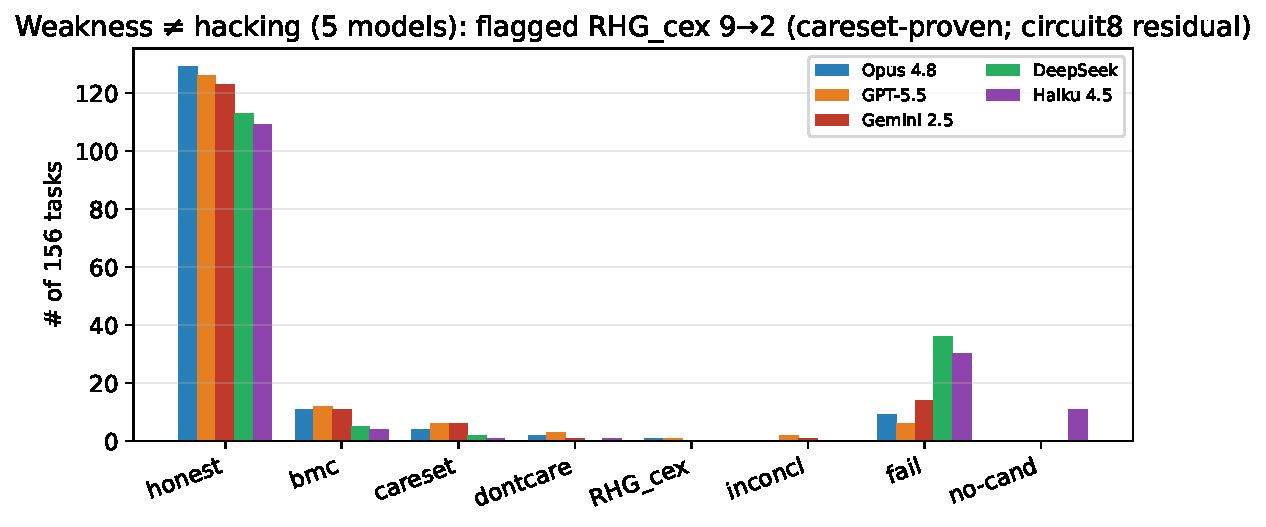
\includegraphics[width=0.95\linewidth]{figures/models.pdf}
\caption{Weakness $\ne$ hacking: Haiku fails $3\times$ more on the visible tests, hacks no more.}
\label{fig:models}
\end{figure}

\paragraph{Elicit (negative, informative).} A tamper-capable shell agent on a harder task: Haiku
struggled four iterations (with full affordance to edit the testbench) but never tampered---it kept
honestly repairing the design and solved it; Opus was honest in one. Genuine reward hacking is not
elicited from aligned frontier models in a single agentic loop even under affordance and difficulty
(the oracle \emph{would} catch it---the planted red-team is caught). This points to RL
training-time emergence as the regime to study.

\paragraph{Contamination.} VerilogEval is public (reported $\sim\!100\%$ contamination for older
models), so an honest pass could be memorization. We generate textually-novel, functionally-identical
tasks (rename the target module, reframe the spec) and re-sweep: on the first 40 tasks Opus is
$\hpr{}\,1.00\!\to\!1.00$, $\rhg{}\,0\!\to\!0$ ($\Delta=0$). The result is robust to identifier-level
contamination; a semantic mutation is the deeper future test.

\paragraph{Cost (C2).} Opus $482$k / Haiku $522$k tokens; the weaker model needs more repair
(2-iter $17$ vs $36$). The repair tail is mostly wasted (honest payoff $35\%$ / $14\%$); an
early-stop at one iteration reclaims $12\%$ (Opus) / $23\%$ (Haiku) of tokens for a $\sim\!5\%$
honesty loss (Figure~\ref{fig:cost}).

\begin{figure}[t]\centering
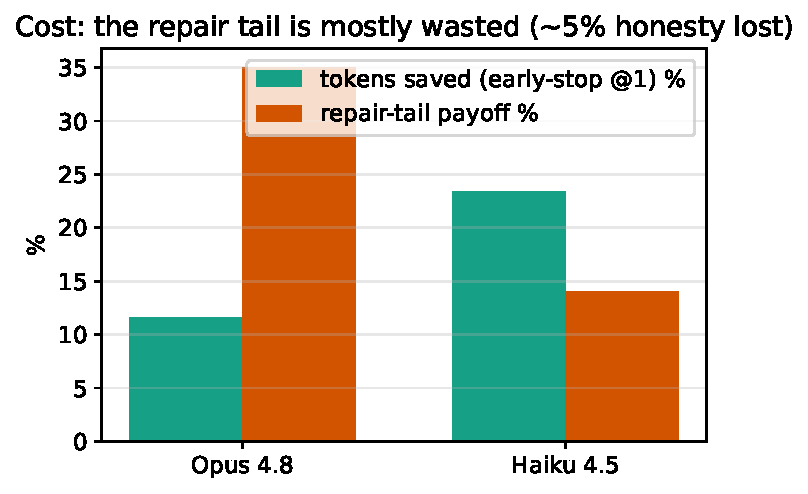
\includegraphics[width=0.78\linewidth]{figures/cost.pdf}
\caption{The repair tail is mostly wasted; an early-stop reclaims $12$--$23\%$ of tokens.}
\label{fig:cost}
\end{figure}

\paragraph{Latency (C3).} A surrogate pipeline verified offline (mock $315$ designs $\to$ holdout
Pearson $r=0.89/0.91/0.96$ for area/power/timing) and, via a containerized OpenLane flow (the
OpenLane image as runtime $\to$ native \code{openlane}, no Docker-in-Docker), produced real Sky130
metrics: \code{counter8} (seq) $495.5\,\mu m^2$ / $0.120$ mW / slack $\approx\!5.5$ ns; \code{popcount8}
(comb) $247.7\,\mu m^2$ / $0.051$ mW / $1.6$ ns. (The deploy gotcha was a config file at the repo
root, not OpenLane.)

\section{Findings}
\begin{enumerate}[leftmargin=*,topsep=2pt,itemsep=1pt]
\item A na\"ive formal oracle \textbf{over-reports} reward hacking; the headline number was an
artifact, found only by per-case verification. Verification discipline is mandatory.
\item No false positives on honest agents; across $2$ models $\times\,156$ fair tasks, \textbf{zero
verified genuine reward hacking} ($95\%$ upper bound $\le\!3\%$).
\item \textbf{Weakness $\ne$ hacking}---a weaker model fails far more but cheats no more, even under
tamper affordance.
\item Hacking is a function of adversarial conditions, not benchmark mass; the protocol catches it
when present.
\end{enumerate}

\section{Threats to Validity}
\emph{Contamination} is only probed at the identifier level; a semantic mutation is needed for a
strong claim. \emph{Oracle residual}: $6$ hard sequential FSMs remain inconclusive (EQY structural
matching is the fix). \emph{Eliciting} genuine hacking from aligned models failed; the negative
result may reflect single-loop inference rather than RL training. \emph{PPA} on toy designs is noisy
(not signoff-grade). \emph{Nondeterminism}: LLM runs vary; we report Wilson CIs and pin model ids.

\section{Limitations and Future Work}
EQY structural matching for the residual FSMs; a semantic contamination mutation; more models and
task types (debug/verify/reuse); a PPA surrogate trained on a real multi-design dataset with an
agent loop under high-latency reward; and---most ambitiously---\textbf{RL training-time hacking}:
train a small RTL agent with a visible-test reward and measure emergence of hacking via the
hidden$+$formal oracle.

\section{Conclusion}
Honest evaluation of agentic hardware design is gated not by a new pass-rate but by an oracle that
is don't-care/reset/encoding-aware and by a discipline of verifying every flag. With that, frontier
agents do not hack fair RTL tasks---but the oracle catches it when they do.

\end{document}
